\section{Introduction}
\label{sec:chap_3_introduction}

At the end of the previous chapter, we introduced a concept called phase-mixing. We saw that very short-length-scales can build up when Alfv\'en waves propagate along field lines with different Alfv\'en travel times. Since each field line has different Alfv\'en travel times, this can lead to waves moving out of phase with their neighbours. This suggests that the ideal assumption we made in the previous chapter may no longer be valid. Moreover, it has been suggested in, for example, \citet{Heyvaerts1983} that phase-mixed Alfv\'en waves could play a significant role in coronal heating.

Phase mixing has been researched extensively since \citet{Heyvaerts1983} first proposed it as a coronal heating mechanism. For example, \citet{Browning1984}, expanded on the \citet{Heyvaerts1983} work related to the Kelvin-Helmholtz instability. They show that standing phase-mixed Alfv\'en waves are unstable to the Kelvin-Helmholtz instability and will undergo a turbulent cascade, leading to enhanced dissipation of energy. In for example, \citet{DeMoortel2002} and \citet{Smith2007} they study phase mixing in a stratified and divergent magnetic field. \citet{Similon1989} and \citet{Howson2019} study phase mixing in a complex magnetic field. \citet{Hood1997,Hood2002} investigate phase mixing in coronal holes and calculate a self-similar solution which enables them to analyse a more general class of solutions. They find that a single pulse decays algebraically rather than exponentially. Phase mixing has been investigated in 3D \citep{Magyar2017} and 3D coronal loops \citep{Pagano2017,Pagano2018}.

In this chapter, we aim to answer whether the phase-mixing of Alfv\'en waves plays an important or negligible role in coronal heating? To help answer this question, we introduce a term called the heating rate per unit of wave energy in a loop, denoted with $\gamma$. We define $\gamma$ as the ratio of the integrated time-averaged heating rate along a loop over the wave energy of the loop, i.e.
\begin{equation}
    \gamma = \frac{\left\langle\int_C \vec{\sigma}_{Brag}:\grad{u} + j^2/\sigma dl\right\rangle}{\frac{1}{2}\left\langle\int_C \rho u^2 + b^2 dl\right\rangle},
\end{equation}
where $C$ is a contour of a given coronal loop and $\langle\rangle$ denotes the time average. Note that $\gamma$ is closely related to the damping coefficient used in the equation to describe damped harmonic oscillators. The equation for a damped harmonic oscillator, with amplitude $x(t)$, is given by
\begin{equation}
    \dv[2]{x}{t}+\gamma_0\dv{x}{t}+\omega_0^2 x = 0.
\end{equation}
Multiplying through by $\dv*{x}{t}$ gives
\begin{equation}
    \dv{}{t}\qty[\frac{1}{2}\qty(\dv{x}{t})^2+\frac{1}{2}\omega_0^2 x] = -\gamma_0 \qty(\dv{x}{t})^2.
\end{equation}
Note that the time average of the potential energy, $\langle \omega_0^2 x^2 / 2 \rangle$, is approximately equal to the time average of the kinetic energy, $\langle (\dv*{x}{t})^2/2\rangle$, therefore, the heating rate over the kinetic and potential energy is given by
\begin{equation}
    \gamma_0 \approx \frac{\gamma_0\langle (\pdv*{x}{t})^2\rangle}{\frac{1}{2}\langle(\pdv*{x}{t})^2+\omega_0^2x^2\rangle}.
\end{equation}
Therefore, $\gamma$ and $\gamma_0$ satisfy very similar definitions, which explains why $\gamma$ is closely related to the waves' damping rate. Note that \citet{Hollweg1984a,Hollweg1984b} uses a very similar idea to $\gamma$ except they use a quantity called the quality factor, from resonance theory, which is approximately given by $\omega / \gamma$, where $\omega$ is the angular frequency of a wave. We focus on using $\gamma$ because it is easier to apply to a system in which multiple frequencies are excited. \citet{Arregui2015} also discusses a similar idea. He argues (through an order magnitude analysis) that phase mixing could take too long to reach the required length scales for the heating rate to become important.

We can estimate the conductive and radiative losses \citep{Withbroe1977} and the wave energy \citep{McIntosh2011,McIntosh2012} in the corona. Using these values, we can approximate the value $\gamma$ needs to satisfy for the conductive and radiative energy losses to be balanced by the viscous and Ohmic dissipation of the observed waves. This gives the required value of $\gamma$ for coronal heating and we will compare it with the value of $\gamma$ predicted by phase-mixing theory. This is how we will test if phase mixing can play a significant role in coronal heating. In Section \ref{sec:chap_3_coronal_heating} we estimate an upper bound for the $\gamma$ predicted by phase-mixing theory by ensuring any simplifications made act to increase the value of $\gamma$. If our upper bound is too small, we can conclude that phase-mixing plays a negligible role in coronal heating. If the upper bound is equal to or larger than the required $\gamma$ then this means phase-mixing could play an important role. However, we would need a more realistic model to know for sure. In this section, we will calculate the required value of $\gamma$ in a closed loop. 

We can estimate the conductive and radiative losses in a closed coronal loop via a theoretical and observational approach. We will first calculate the theoretical energy losses and then check them with the observations given by \citet{Withbroe1977}. If we assume the radiative loss function can be approximated with
\begin{equation}
    Q(T) = \chi T^{-1/2},
\end{equation}
where $\chi=10^{-32}\si{.K^{1/2}.W.m^3}$, then \citet{Priest2014} shows that to maintain a loop with a uniform pressure, $p$, with a uniform heating rate, $H_c$, then $H_c$ must satisfy
\begin{equation}
    \label{eq:coronal_heating_rate_per_unit_volume}
    \begin{aligned}
    H_c &= \frac{7}{8}\frac{\chi}{k_B^2}\frac{p^2}{T_{max}^{5/2}} \\
    &\approx 4.59\times10^{-6}\qty(\frac{\chi}{10^{-32}\si{.K^{1/2}.W.m^3}})\qty(\frac{p}{10^{-2}\si{.Pa}})^2\qty(\frac{10^6\si{.K}}{T_{max}})^{5/2}\si{.W.m^{-3}}
    \end{aligned}
\end{equation}
Table \ref{tbl:energy_losses_corona_chromosphere} shows the power losses due to conduction, radiation and solar wind per unit area in the corona. The table gives the power per unit area, whereas our theoretical calculation is per unit volume. Therefore, we need to integrate our theoretical calculation in the radial direction. We model the temperature as uniform in the radial direction and assume the pressure satisfies hydrostatic balance. In other words, we assume that
\begin{equation}
    p=p_0\exp(-r/h),
\end{equation}
where $h$ is the pressure scale height given by Equation \eqref{eq:pressure_scale_height}. Note that for typical values ($m=m_p/2$, $g_{\odot}=274\si{.m^2.s^{-1}}$) the pressure scale height is given by
\begin{equation}
    h = 1.51\times10^8\qty(\frac{T}{10^6\si{.K}})\si{.m}
\end{equation}
Most heating will occur within a height $2h$ of the solar surface, the radius of the Sun is about $0.70\times10^9\si{.m}$ \citep{sun_vital_statistics} which is greater than $h$. Therefore, the error associated with approximating the gravitational field strength as uniform will be small. 
We now need to integrate Equation \eqref{eq:coronal_heating_rate_per_unit_volume} in the radial direction from $r_0$ to $r_1$, where $r_0$ gives the radial coordinate of the base of the corona and $r_1$ gives the coordinate of the top of the corona. The height of the corona is not clearly defined, however, we know that $r_1-r_0\gg h$, therefore, we can approximate $r_1\rightarrow \infty$. Hence, the integral of Equation \eqref{eq:coronal_heating_rate_per_unit_volume} is given by
\begin{equation}
    \begin{aligned}
    \int_{r_0}^\infty H_c \, dr &= \frac{h}{2}\frac{7}{8}\frac{\chi}{k_B^2}\frac{p(r_0)^2}{T_{max}^{5/2}} \\
    &\approx 3.47\times10^{2}\qty(\frac{\chi}{10^{-32}\si{.K^{1/2}.W.m^3}})\qty(\frac{p(r_0)}{10^{-2}\si{.Pa}})^2\qty(\frac{10^6\si{.K}}{T_{max}})^{3/2}\si{.W.m^{-2}}
    \end{aligned}
\end{equation}
where $r_0$ gives the radial coordinate of the base of the corona. Note that Table \ref{tbl:energy_losses_corona_chromosphere}, shows that the energy losses are in the range $[3\times10^2,10^4]\si{.W.m^{-2}}$ and our calculation above lies in this range. Therefore, the theoretical and observational calculations are in agreement. 

In \citet{McIntosh2011,McIntosh2012}, they observe velocity wave amplitudes, $u_0$, in the quiet sun of around $20\si{.km.s^{-1}}$ and in active regions of around $5\si{.km.s^{-1}}$. We can use this data to estimate the corona's wave energy by assuming the time-averaged kinetic energy associated with the waves equals the time-averaged magnetic perturbation energy. This gives a wave energy, $E_{wave}$, of approximately
\begin{equation}
    \label{eq:chap_3_observed_wave_energy}
    \begin{aligned}
    E_{wave} &\approx \rho \langle u_0 \rangle^2 \\
    &\approx10^{-4}\qty(\frac{\rho}{10^{-12}\si{.kg.m^{-3}}}) \qty(\frac{\langle u_0 \rangle}{10^4 \si{.m.s^{-1}}})^2\si{.J.m^{-3}}.
    \end{aligned}
\end{equation}
Therefore, the value $\gamma$ needs to satisfy for the conductive and radiative energy losses to be balanced by the viscous and Ohmic dissipation of the observed waves is given by
\begin{equation}
\label{eq:required_gamma}
\begin{aligned}
    \gamma &= \frac{H_c}{E_{wave}} \\
    &= \frac{7}{2}\frac{\chi}{m_p^2}\frac{\rho}{T_{max}^{1/2}}\frac{1}{\langle u_0\rangle^2} \\
    &\approx1.25\times10^{-1}\qty(\frac{\rho}{10^{-12}\si{.kg.m^{-3}}})\qty(\frac{10^6\si{.K}}{T_{max}})^{1/2}\qty(\frac{10^{4}\si{.m.s^{-1}}}{\langle u_0 \rangle})^2\si{.s^{-1}}.
\end{aligned}
\end{equation}
Therefore, the $\gamma$ predicted by phase-mixing needs to be of the order $10^{-1}\si{.s^{-1}}$ for it provide an important role in coronal heating.

\section{Model and equations}

This chapter will model perturbations on a background medium. We assume the system is linear and we make the same assumptions as described by Equations \eqref{eq:linear_assumotion_v}-\eqref{eq:linear_assumotion_rho}. We will model the background quantities as uniform in $z$. The background magnetic field points in the $z$-direction, i.e.
\begin{equation}
    \tag{\ref{eq:background_field}}
    \vec{B}_0 = B_0\vec{\hat{z}}.
\end{equation}
We model the background Alfv\'en speed to be a function of $x$, i.e. $v_A=v_A(x)$.

We assume the $y$-direction is invariant, i.e. $\pdv*{}{y}=0$. This prevents mode coupling between $u_x$ and $u_y$. \citet{Parker1991} argues that this mode conversion is important and should not be neglected. However, in Chapter \ref{chap:resonant_absorption_in_an_oblique_field} we find that at resonant locations the mode conversion is one-way from fast to Alfv\'en waves. Therefore, the results presented in this chapter are relevant at these resonant locations (which are discussed in greater detail in Chapter \ref{chap:resonant_absorption_in_an_oblique_field}). Some coronal arcades have an approximate invariant direction, and some flux tubes can be azimuthally invariant. Assuming $\pdv*{}{y}=0$ prevents the development of MHD instabilities. In \citet{Heyvaerts1983}, they show that, for $\pdv*{}{y}\ne0$, standing phase-mixed Alfv\'en waves are unstable to the Kelvin-Helmholtz and tearing instabilities. Also, $\pdv*{}{y}=0$ prevents viscous heating due to gradients in the $y$-direction. If we assume $\vec{u}=u(x,y,z,t)\vec{\hat{y}}$ and $\vec{b}=b(x,y,z,t)\vec{\hat{y}}$ then the viscous heating associated with $\vec{W}^{(0)}$ becomes
\begin{equation}
    \eta_0 \vec{W}^{(0)}:\grad{\vec{u}} = \frac{\eta_0}{3}\qty(\pdv{u}{y})^2,
\end{equation}
where $\vec{W}^{(0)}$ is given by Equation \eqref{eq:braginskii_viscous_stress_tensor}.

We solve for the $y$-component of the velocity, given by
\begin{equation}
    \tag{\ref{eq:y_component_of_u}}
    \vec{u}(x,z,t) = u(x,z,t)\vec{\hat{y}},
\end{equation}
and the $y$-component of the perturbed magnetic field, given by
\begin{equation}
    \tag{\ref{eq:y_component_of_b}}
    \vec{b}(x,z,t) = b(x,z,t)\vec{\hat{y}}.
\end{equation}

The $y$-component of the linearised momentum equation, see Equation \eqref{eq:momentum}, with gravity neglected, see Equation \eqref{eq:ignore_gravity}, is given by
\begin{equation}
    \label{eq:chap_3_momentum_eqn1}
    \begin{aligned}
    \pdv{u}{t} &= \frac{v_A^2(x)}{B_0}\pdv{b}{z} + \frac{1}{\rho}\vec{\hat{y}}\cdot\div{\vec{\sigma}_{Brag}} \\
    &\approx\frac{v_A^2(x)}{B_0}\pdv{b}{z} +\frac{\eta_1}{\rho} \pdv[2]{u}{x} + \frac{\eta_2}{\rho} \pdv[2]{u}{z}.
    \end{aligned}
\end{equation}
where $\vec{\sigma}_{Brag}$ is given by Equation \eqref{eq:braginskii_viscous_stress_tensor}, the plasma pressure and magnetic pressure terms are set to zero because the $y$-direction is invariant. Note that when calculating $\div\vec{\sigma}_{Brag}$, we ignored the derivatives associated with the coefficients, $\eta_0,\eta_1, ...$ etc. as we expect our waves to phase mix and so we expect $\abs{\pdv*{u}{x}/u}\gg\abs{\pdv*{\eta_0}{x}/\eta_0}$. The equations above shows that after linearising the Braginskii viscous tensor, the contribution from the parallel component, $\eta_0\vec{W}^{(0)}$, and the drift terms, $\eta_3\vec{W}^{(3)}$, $\eta_4\vec{W}^{(4)}$ is zero. This result and a discussion on the linearised Braginskii viscous stress tensor are given in, for example, \citet{Ruderman2000,Mocanu2008}. Equations \eqref{eq:braginskii_eta_0} to \eqref{eq:braginskii_eta_2} show that $\eta_0$ is usually much greater than $\eta_1$ and $\eta_2$. Equation \eqref{eq:proton_gyrofrequency_times_collision_time} shows that we estimate $\eta_0$ to be a factor $10^{10}$ greater. By linearising the viscous stress tensor we could be neglecting the dominant term. However, this chapter aims to just study just linear waves, in Section \ref{sec:chap_3_coronal_heating} we investigate parameter space in which this linearization is justified. We intend to study phase mixing, which is a concept we introduced in Section \ref{sec:phase_mixing}, so we make another assumption which is to assume $\pdv*{}{x}\gg\pdv*{}{z}$. Therefore, we simplify Equation \eqref{eq:chap_3_momentum_eqn1} further to give
\begin{equation}
    \label{eq:chap_3_momentum_eqn2}
    \pdv{u}{t}=\frac{v_A^2(x)}{B_0}\pdv{b}{z} +\nu\pdv[2]{u}{x},
\end{equation}
where we set $\nu = \eta_1/\rho$ to keep the notation tidy.

The $y$-component of the linearised induction equation, see Equation \eqref{eq:induction_equation}, is given by
\begin{equation}
    \pdv{b}{t} = B_0\pdv{u}{z}+\eta\nabla^2 b - \underbrace{\vec{\hat{y}}\cdot\curl(\frac{1}{n_e e}\vec{j}\cross\vec{B})}_{\text{Hall term}}.
\end{equation}
Like in the previous paragraph, we simplify this equation further by assuming that $\pdv*{}{x}\gg\pdv*{}{z}$ to give 
\begin{equation}
    \label{eq:chap_3_induction}
    \pdv{b}{t} = B_0\pdv{u}{z}+\eta\pdv[2]{b}{x}.
\end{equation}
Note that we have neglected the Hall term because it is dependent on derivatives which are parallel to the background magnetic field. In, for example, \citet{Threlfall2017} they investigate the effects of the Hall term on phase mixing. They find that the hall terms' introduction causes wave dispersion which reduces the heating rate per unit of wave energy, $\gamma$. We aim to show that linear phase mixed Alfv\'en waves at observed wavelengths have an insufficient $\gamma$ to heat the corona. Therefore, if $\gamma$ is insufficient without the Hall term, we know it must be insufficient with the Hall term.

Substituting Equation \eqref{eq:chap_3_induction} into the time derivative of Equation \eqref{eq:chap_3_momentum_eqn2} gives
\[\pdv[2]{u}{t}=v_A^2(x)\pdv[2]{u}{z}+v_A^2(x)\pdv[2]{}{x}\qty(\frac{\eta}{B_0}\pdv{b}{z})+\nu\pdv{}{t}\pdv[2]{u}{x}.\]
Note that
\[\begin{aligned}
\pdv[2]{}{x}\qty(\frac{\eta}{B_0}\pdv{b}{z}) &= \pdv[2]{}{x}\qty[\frac{\eta}{v_A^2(x)}\qty(\pdv{u}{t} - \nu \pdv[2]{u}{x})] \\
&\approx \frac{\eta}{v_A^2(x)}\pdv{}{t}\pdv[2]{u}{x},
\end{aligned}\]
where we assume that $\eta$ and $\nu$ are small factors such that their products are negligible. Moreover, we assume that $\abs{\pdv*{u}{x}/u}\gg\abs{\pdv*{v_A}{x}/v_A}$ and so we get the approximation above. Using the above two equations we get
\begin{equation}
    \label{eq:wave_diffusion_equation}
    \pdv[2]{u}{t}-v_A^2(x)\pdv[2]{u}{z}= (\eta+\nu)\pdv{}{t}\pdv[2]{u}{x}.
\end{equation}

Equation \eqref{eq:chap_3_momentum_eqn2} can be written as
\[\pdv{u}{t}=v_A(x)\pdv{\hat{b}}{z}+\nu\pdv[2]{u}{x},\]
where
\begin{equation}
    \hat{b}(x,z,t) = \frac{v_A(x)}{B_0}b(x,z,t).
\end{equation}
Also if we assume $\abs{\pdv*{b}{x}/b}\gg\abs{\pdv*{v_A}{x}/v_A}$ then we can approximate Equation \eqref{eq:chap_3_induction}, multiplied by $v_A(x)/B_0$ as 
\[\pdv{\hat{b}}{t}=v_A(x)\pdv{u}{z}+\eta\pdv[2]{\hat{b}}{x}.\]
Combining the above equations gives
\begin{equation}
    \label{eq:advection_diffusion_elsasser}
    \pdv{\mathcal{Z}^\pm}{t} \mp  v_A(x)\pdv{\mathcal{Z}^\pm}{z} = \nu_+ \pdv[2]{Z^\pm}{x} + \nu_-\pdv[2]{Z^\mp}{x},
\end{equation}
with $Z^{\pm}$ is given by 
\begin{equation}
    \tag{\ref{eq:elsasser_z}}
    \mathcal{Z}^\pm(x,z,t) = u(x,z,t) \pm \frac{v_A(x)}{B_0}b(x,z,t),
\end{equation}
and $\nu_{\pm}$ is given by
\begin{equation}
    \nu_\pm = \frac{1}{2}(\eta\pm\nu),
\end{equation}
where we assumed that $\abs{\pdv*{b}{x}/b}\gg\abs{\pdv*{v_A}{x}/v_A}$.

In this chapter, we will solve the above equations for various boundary conditions. In Section \ref{sec:chap_3_open_loop} we solve the above equations for the case where the boundaries are open, in Section \ref{sec:chap_3_closed_loop} we consider a closed-loop and in Section \ref{sec:chap_3_leaky_loop} we study a leaky loop. In all sections, we will have a driver at the bottom boundary ($z=0$) given by
\begin{equation}
    \label{eq:driver_chap_3}
    \begin{aligned}
    u(x,0,t) &= f_{driv}(x,t) \\
    &= f_0\exp(i\omega t).
    \end{aligned}
\end{equation}
We will impose Neumann boundary conditions in $x$, i.e.
\begin{equation}
    \label{eq:neumann_bcs_chap_3}
    \left.\pdv{u}{x}\right|_{x=x_{min}}=\left.\pdv{u}{x}\right|_{x=x_{max}}=0.
\end{equation}
Our initial conditions are
\begin{equation}
    u(x,z,0) = b(x,z,0) = 0.
\end{equation}
For our numerical solutions, the background Alfv\'en speed is given by
\begin{equation}
    \label{eq:background_vA_chap_3}
    v_A(x) = v_{A0}\qty[1 + \frac{x}{a_0}],
\end{equation}
however, for our analytic solutions we will assume the more general form, namely, $v_A=v_A(x)$.

We seek the steady-state solution, where the solution oscillates at the driver frequency. Therefore, we assume a time-dependence of the form $\exp(i\omega t)$ implicitly. Therefore,
Equation \eqref{eq:wave_diffusion_equation} can be written as
\begin{equation}
    \label{eq:method_of_lines_eqn_u}
    \boxed{-i\omega(\eta+\nu)\pdv[2]{u}{x} = \omega^2u + v_A^2\pdv[2]{u}{z},}
\end{equation}
and Equation \eqref{eq:advection_diffusion_elsasser} gives
\begin{equation}
    \label{eq:chap_3_method_of_lines_eqn}
     \boxed{\pdv{\mathcal{Z}^\pm}{z} = \frac{1}{v_A(x)}\qty{\pm i\omega Z^{\pm} + \nu_+ \pdv[2]{Z^\pm}{x} + \nu_-\pdv[2]{Z^\mp}{x}}.}
\end{equation}

\section{Open loop}
\label{sec:chap_3_open_loop}

This section aims to calculate solution to Equation \eqref{eq:chap_3_method_of_lines_eqn} analytically and numerically, for an open loop. We assume the loop contains only waves propagating in the positive $z$-direction so $\mathcal{Z}^+=0$.

\subsection{Analytic solution}

To solve Equation \eqref{eq:chap_3_method_of_lines_eqn} analytically we will use the method of multiple scales, where $\eta+\nu$ gives the small parameter. Since $\mathcal{Z}^+=0$ $\implies$ $u = \mathcal{Z}^{-}/2$. Substituting this into Equation \eqref{eq:chap_3_method_of_lines_eqn} gives
\begin{equation}
    \pdv{u}{z}+ik_z(x)u=\frac{\eta+\nu}{2v_A(x)}\pdv[2]{u}{x},
\end{equation}
where
\begin{equation}
    k_z(x) = \frac{\omega}{v_A(x)}.
\end{equation}
We assume $u(x,z)$ takes the form of the following asymptotic series
\begin{equation}
    u(x,z_0,z_1) = u_0(x,z,\epsilon z) + \epsilon u_1(x,z,\epsilon z) + \epsilon^2 u_2(x,z,\epsilon z) + ...\,.
\end{equation}
where $u$ has a shorter length-scale dependence, $z_0$, given by
\begin{equation}
    z_0 = z
\end{equation}
and a longer length-scale dependence, $z_1$, given by
\begin{equation}
    z_1 = \epsilon z.
\end{equation}
The zeroth order equation is given by
\begin{equation}
    \pdv{u_0}{z}+ik_z(x)u_0=0.
\end{equation}
Solving with the boundary condition,
\begin{equation}
    u(x,0)=f_0,
\end{equation}
gives
\begin{equation}
    \label{eq:u_0_short_timescale}
    u_0(x,z,z_1) = f_0\exp[-ik_z(x)z]A(z_1).
\end{equation}
Note that
\begin{equation}
    \pdv{u}{z} = \pdv{u}{z_0} + \epsilon \pdv{u}{z_1}.
\end{equation}
Hence, the first order equation is given by
\begin{equation}
    \pdv{u_1}{z}+ik_z(x)u_1 = -\pdv{u_0}{z_1}+\frac{\eta+\nu}{2\epsilon v_A}\pdv[2]{u_0}{x}.
\end{equation}
In order to eliminate secular terms we equate the right-hand side of the above equation to be zero which gives
\begin{equation}
    \pdv{u_0}{z_1}-\frac{(\eta+\nu)}{2\epsilon v_A}\pdv[2]{u_0}{x}=0.
\end{equation}
Evaluating the $x$-derivative gives
\begin{equation}
    \pdv{u_0}{z_1}+\qty(\dv{k_z}{x})^2\frac{(\eta+\nu)}{2\epsilon^3 v_A}z_1^2u_0=0.
\end{equation}
In order to make both terms the same order, we choose $\epsilon = (\eta+\nu)^{1/3}$. This has the general solution,
\begin{equation}
    \label{eq:u_0_long_timescale}
    u_0(x,z,z_1) = C(z)\exp[-\frac{(\dv*{k_z}{x})^2}{6v_A}z_1^3].
\end{equation}
Therefore, combining Equation \eqref{eq:u_0_short_timescale} with \eqref{eq:u_0_long_timescale} gives to leading order
\begin{equation}
    \label{eq:leading_order_phase_mixed_soln}
    \begin{aligned}
    u(x,z) &= f_0\exp[-k_z(x)z]\exp[-\qty(\dv{k_z}{x})^2\frac{\eta+\nu}{6v_A}z^3] \\
    &= f_0\exp[-k_z(x)z]\exp[-\qty(\dv{v_A}{x})^2\frac{\eta+\nu}{6v_A^5}\omega^2 z^3] \\
    &= f_0\exp[-k_z(x)z]\exp[-\frac{\eta+\nu}{6\omega a^2}k_z^3 z^3], \\
    \end{aligned}
\end{equation}
where 
\begin{equation}
    \label{eq:length_scale_alfven_travel_time}
    a(x) = \frac{v_A(x)}{\dv*{v_A}{x}},
\end{equation}
which gives a measure of the length-scale of the Alfv\'en travel time.
Since we approximated $Z^{+}=0$, we know that $b(x,z,t) = -B_0 u(x,z,t) / v_A(x)$, therefore, to leading order
\begin{equation}
    \label{eq:leading_order_phase_mixed_soln_b}
    \begin{aligned}
    b(x,z) &= B_0\frac{f_0}{v_A(x)}\exp[i(\omega t-k_z(x)z)]\exp[-\frac{\eta+\nu}{6\omega a^2}k_z^3 z^3].
    \end{aligned}
\end{equation}
Note that the length-scale of the envelope, $L_{ph}$, is given by
\begin{equation}
    \label{eq:phase_mixed_z_length_scale}
    L_{ph}(x) = \qty[\frac{6\omega a^2}{\eta+\nu}]^{1/3}\frac{1}{k_z}.
\end{equation}
In Section \ref{sec:phase_mixing}, Equation \eqref{eq:phase_mixing_du_dx}, we showed that the effective wavenumber in $x$, $k_x^*$, is given by
\begin{equation}
    \label{eq:kx_star}
    \begin{aligned}
    k_x^*(x) &= \omega \dv{v_A}{x}\frac{z}{v_A^2} \\
    &=k_z z / a.
    \end{aligned}
\end{equation}
Therefore, at $z=L_{ph}$, $k_x^*$ is given by
\begin{equation}
    \label{eq:phase_mixed_x_length_scale}
    k_x^*= \qty[\frac{6\omega }{(\eta+\nu)a}]^{1/3}.
\end{equation}

In Section \ref{sec:intro_assumptions} we showed that in the strong field limit, for collisional transport theory to be valid, Equation \eqref{eq:length_scale_condition_perpendicular} needs to be satisfied. Therefore, we require
\begin{equation}
    \frac{2\pi}{k_x^*} \gg \sqrt{\lambda_{Ti} r_e}.
\end{equation}
For typical values, the phase-mixed length scale in $x$ is given by
\begin{equation}
    \frac{2\pi}{k_x^*}=1.1\qty(\frac{\pi\times10^{-2}\si{.Hz}}{\omega})\qty(\frac{\eta+\nu}{1\si{.m^2.s^{-1}}})^{1/3}\qty(\frac{a}{1\si{.Mm}})^{1/3}\si{.Mm}.
\end{equation}
This shows Equation \eqref{eq:length_scale_condition_perpendicular} is usually satisfied.

\subsection{Numerical solution}

Our goal now is to to check the accuracy of Equation \eqref{eq:leading_order_phase_mixed_soln} by solving Equation \eqref{eq:chap_3_method_of_lines_eqn} using the method of lines. We discretize in $x$, i.e. we replace the $x$-derivatives in Equation \eqref{eq:chap_3_method_of_lines_eqn} with finite difference approximations. This gives a set of ODEs in the $z$ which we solve as an initial value problem using \texttt{solve\_ivp} in \citet{SciPy2020}. We assume the domain contains only waves propagating in the positive $z$-direction and set $Z^{+}=0$. We choose the $x$-domain to be given by $x\in[-l_x,l_x]$, 
where
\[l_x = \frac{10}{k_x^*}.\]
The Alfv\'en speed is given by Equation \eqref{eq:background_vA_chap_3} and the driver is given by  Equation \eqref{eq:driver_chap_3}.

\begin{figure}
    \centering
    \vspace{-20pt}
    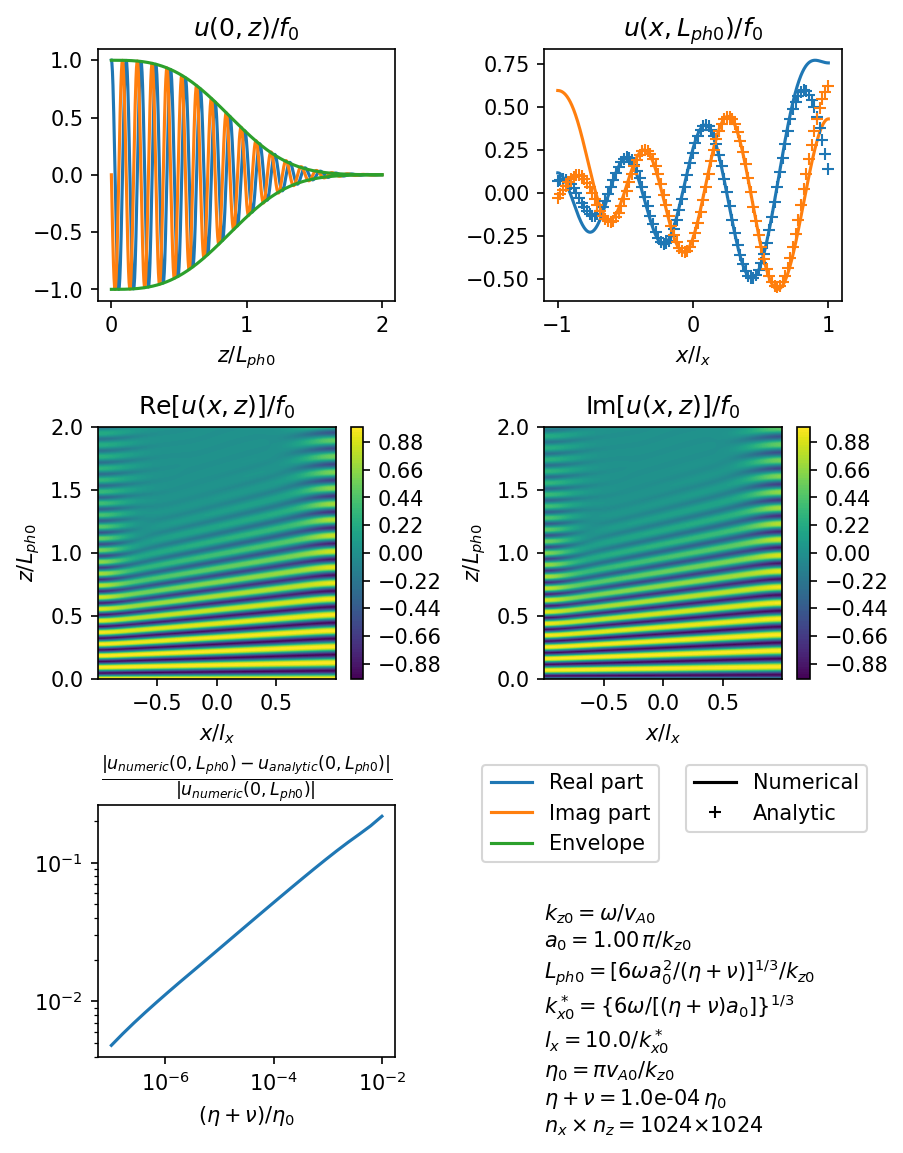
\includegraphics[width=\textwidth,height=0.85\textheight,keepaspectratio]{figures/chapter03/phase_mixing_open_loop.png}
    \vspace{-10pt}
    \caption{This figure shows plots of the velocity perturbation of phase-mixed Alfv\'en waves in an open loop. The top-left shows a plot along $z$ at $x=0$, where the green curve shows the envelope which we calculated using Equation \eqref{eq:velocity_envelope}. The top-right plot shows the analytic and numerical solutions along $x$ at $z=L_{ph0}$. The middle-row shows contour plots of the real and imaginary parts. The bottom-left plots the relative error between the analytic and numerical solutions at $x=0$, $z=L_{ph0}$ as a function of $\eta+\nu$. In the bottom-right, we show some of the parameters we used. The code used to make this figure is available on GitHub in the following directory:\newline
    \texttt{$\rightarrow$ Python/Chapter3/open\_loop.py}}
    \vspace{-30pt}
    \label{fig:phase_mxing_open_loop}
\end{figure}

Our goal now is to check that that the numerical solution agrees with the analytic solution. We test this via a graphical approach. In Figure \ref{fig:phase_mxing_open_loop} we plot the velocity perturbation $u$. The top-left shows the velocity along $z$ at $x=0$. The blue and orange curves show the real and imaginary parts, respectively. The green curve shows the envelope, $u_{env}$ which is given by
\begin{equation}
    \label{eq:velocity_envelope}
    u_{env\pm}(x,z) = \pm f_0\exp[-(z/L_{ph})^3],
\end{equation}
which comes from Equation \eqref{eq:leading_order_phase_mixed_soln}. It shows that at $x=0$, to a good approximation, the wave decays with our predicted slope, given by Equation \eqref{eq:leading_order_phase_mixed_soln}. The top-right plot shows the velocity along $x$ at $z=L_{ph0}$, where we show the equation for $L_{ph0}$ in the bottom-right of the figure. The solid line gives the numerical solution and the $+$ symbols give the analytic solution, given by Equation \eqref{eq:leading_order_phase_mixed_soln}. It shows that close to $x=0$, the analytic and numerical solutions show good agreement. However, close to the boundaries, the agreement is poor, and this is because we impose Neumann boundary conditions, see Equation \eqref{eq:neumann_bcs_chap_3}. Our analytic solution works well for open boundary conditions in $x$. However, these are difficult to implement numerically. The middle-row shows contour plots of the real and imaginary parts of the velocity as a function of $x$ and $z$. Finally, the bottom-left shows the relative error between the numerical and analytic solutions at $x=0$ and $z=L_{ph0}$ as a function of $\eta+\nu$. It shows that as we decrease $\eta+\nu$ the error reduces, despite $L_{ph0}$ increasing. In the bottom-right, we show some of the parameters we use, including the grid resolution $n_x\times n_z$.

\section{Closed loop}
\label{sec:chap_3_closed_loop}

In this section we aim to solve Equation \eqref{eq:method_of_lines_eqn_u} for a closed loop, where we impose $u=0$ at the top boundary, i.e.,
\begin{equation}
    u(x,L_z)=0,
\end{equation}
where the domain is given by $z\in[0,L_z]=[0,2l_z]$.

\subsection{Analytic solution}

Using a method of images approach, like that used in Section \ref{sec:closed_loop_sinusoidal_solution}, as well as Equation \eqref{eq:leading_order_phase_mixed_soln}, we calculate the steady-state solution to be
\begin{equation}
    \label{eq:chap_3_closed_loop_phase_mix_soln_u}
    \begin{aligned}
    u(x,z) &= f_0\sum_{k=0}^\infty (-1)^k\exp\qty[-ik_z(x)z_k]\exp[-(z_k / L_{ph})^3] \\
    &= f_0A_\infty(x,z)
    \end{aligned}
\end{equation}
where
\begin{equation}
    z_k = (-1)^k (z-l_z) + (2k+1)l_z,
\end{equation}
and
\begin{equation}
    A_\infty(x,z) = \sum_{k=0}^\infty (-1)^k \exp(-ik_z z_k)\exp[-(z_k / L_{ph})^3].
\end{equation}
Similarly, we calculate the magnetic field to be given by
\begin{equation}
    \label{eq:chap_3_closed_loop_phase_mix_soln_b}
    \begin{aligned}
    b(x,z) &= -B_0\frac{f_0}{v_A}\sum_{k=0}^\infty \exp\qty[-k_z(x)z_k]\exp[-(z_k / L_{ph})^3] \\
    &= -B_0\frac{f_0}{v_A}B_\infty(x,z)
    \end{aligned}
\end{equation}
where
\begin{equation}
    B_\infty(x,z) = \sum_{k=0}^\infty \exp(-ik_z z_k)\exp[-(z_k / L_{ph})^3].
\end{equation}
We are not aware of any method to simplify the summations given by $A_\infty$ and $B_\infty$ further, however, we can approximate them numerically by truncating the series after $N_a$ terms and then calculating the resulting summation numerically, provided $N_a\gg 1$.

\subsection{Numerical solution}

Our goal now is to verify Equations \eqref{eq:chap_3_closed_loop_phase_mix_soln_u} numerically. 
We will convert Equation \eqref{eq:method_of_lines_eqn_u} into a set of ODEs, using the same approach used in Section \ref{sec:chap_2_driven_harmonic_oscillator}. Let
\begin{equation}
    u(x,z) = y(x,z) + f_0\frac{L_z - z}{L_z},
\end{equation}
hence, the boundary conditions for $y$ are
\begin{equation}
    y(x,0)=y(x,L_z)=0.
\end{equation}
We can write Equation \eqref{eq:method_of_lines_eqn_u} as
\[
-i\omega(\eta+\nu)\pdv[2]{y}{x}=\omega^2 y + v_A^2 \pdv[2]{y}{z} + \omega^2f_0\frac{L_z - z}{L_z}.
\]
Note that the we can write the end term as the following Fourier series
\[\omega^2f_0\frac{L_z - z}{L_z} = 2\omega^2f_0\sum_{n=1}^\infty\frac{\sin(k_{zn}z)}{n\pi},\]
where
\begin{equation}
    k_{zn} = \frac{n\pi}{L_z}.
\end{equation}
Let
\begin{equation}
    \label{eq:chap_3_closed_loop_yn}
    y(x,z) = \sum_{n=1}^\infty y_n(x)\sin(k_{zn} z).
\end{equation}
Therefore, each $y_n$ satisfies
\begin{equation}
    \dv[2]{y_n}{x}=i\frac{\omega^2 - v_A^2(x)k_{zn}^2}{\omega(\eta+\nu)}y_n + \frac{2i\omega f_0}{n\pi(\eta+\nu)}.
\end{equation}
We solve this set of ODEs using \texttt{solve\_bvp} in \citet{SciPy2020}. We use the same Alfv\'en speed profile as the last section, namely Equation \eqref{eq:background_vA_chap_3}. We choose the driver frequency, $\omega$, to be given by
 \begin{equation}
     \omega = \frac{\pi v_{A0}}{L_z},
 \end{equation}
 this ensures the driving frequency is equal to the fundamental frequency of the loop at $x=0$.
 Note that we approximate Equation \eqref{eq:chap_3_closed_loop_yn} by truncating the series after $N_h$ terms. We find that the error is small because the solution associated with the fundamental harmonic dominates due to the resonance being excited.
 
\begin{figure}
    \centering
    \vspace{-20pt}
    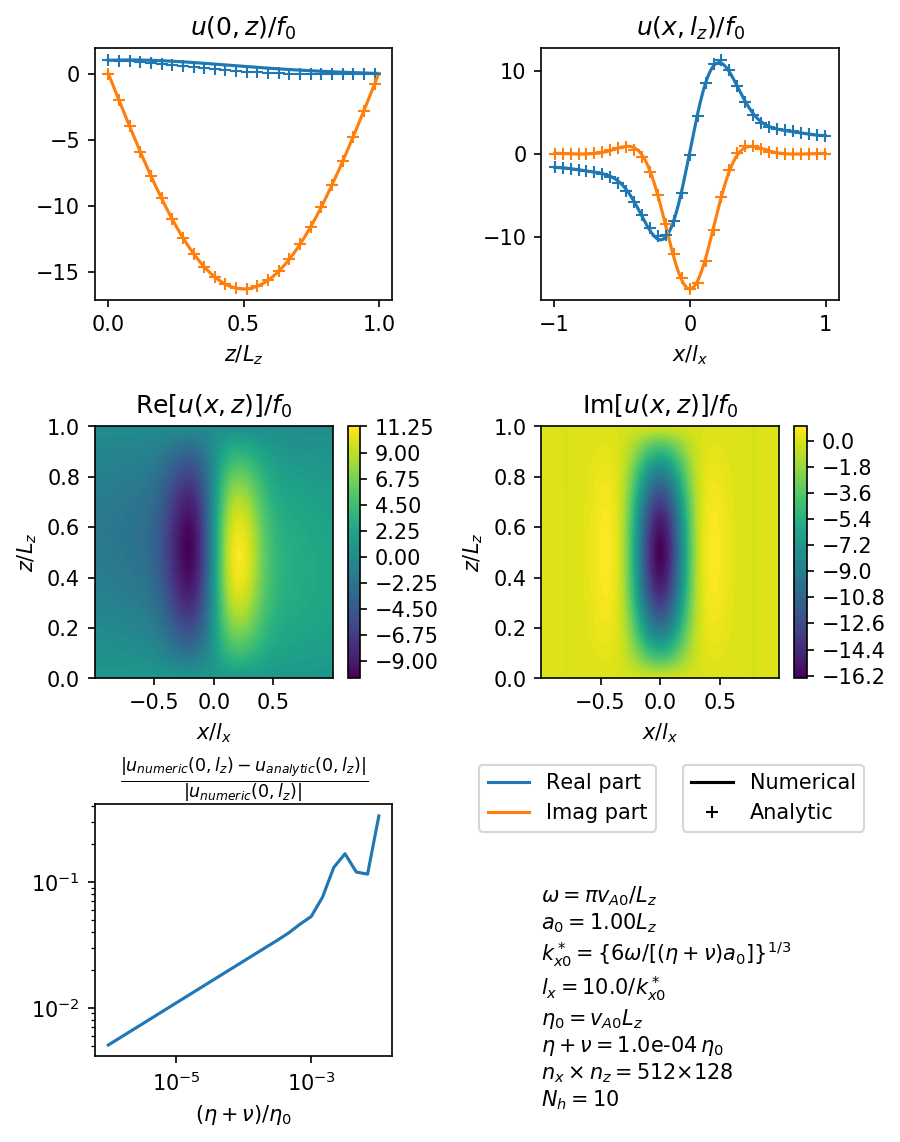
\includegraphics[width=\textwidth,height=0.85\textheight,keepaspectratio]{figures/chapter03/phase_mixing_closed_loop.png}
    \vspace{-10pt}
    \caption{This figure shows plots of the velocity perturbation of phase-mixed Alfv\'en waves in a closed loop. The top-left shows a plot along $z$ at $x=0$. The top-right plot shows the analytic and numerical solutions along $x$ at $z=l_z$. The middle-row shows contour plots of the real and imaginary parts. The bottom-left plots the relative error between the analytic and numerical solutions at $x=0$, $z=l_z$ as a function of $\eta+\nu$. The code used to make this figure is available on GitHub in the following directory:\newline
    \texttt{$\rightarrow$ Python/Chapter3/closed\_loop.py}}
    \label{fig:phase_mixing_closed_loop}
    \vspace{-30pt}
\end{figure}
 
We can now verify Equations \eqref{eq:chap_3_closed_loop_phase_mix_soln_u} via a graphical approach. In Figure \ref{fig:phase_mixing_closed_loop} we plot the velocity perturbation, $u$. The top-left shows the velocity along $z$ at $x=0$. The blue and orange curves show the real and imaginary parts, respectively, see legend in bottom-right of the figure. It shows that the fundamental harmonic dominates the solution because we drive at the field line's fundamental frequency at $x=0$. The top-right plot shows the velocity along $x$ at $z=l_z$, i.e. the middle of the loop. The solid line gives the numerical solution and the $+$ symbols give the analytic solution, given by Equation \eqref{eq:leading_order_phase_mixed_soln}. The imaginary part shows a vertical velocity shear, giving rise to the Kelvin-Helmholtz instability \citep{Heyvaerts1983}. The middle-row shows contour plots of the real and imaginary parts of the velocity as a function of $x$ and $z$. Finally, the bottom-left shows the relative error between the numerical and analytic solutions at $x=0$ and $z=L_{ph0}$ as a function of $\eta+\nu$. It shows that as we decrease $\eta+\nu$, the error reduces.
 
\subsection{Heating rate}
\label{sec:chap_3_closed_loop_heating_rate}
 
In this section, we study the heating rate per unit of wave energy, $\gamma$. Using Equation \eqref{eq:poynting_flux_chap_2} we know that the time-averaged Poynting flux in the $z$-direction, $\langle S_z \rangle$, is given by
\begin{equation}
    \begin{aligned}
    \langle S_z \rangle &= -\frac{B_0}{4\mu}(u\bar{b} + \bar{u}b) \\
    &= \frac{B_0^2f_0^2}{2\mu v_A}\Re(A_\infty\bar{B}_\infty)
    \end{aligned}
\end{equation}
At steady-state, the rate of change of energy in the loop is equal to the loop's heating rate. Therefore, the heating rate is given by the Poynting flux at $z=0$ as the Poynting flux at $z=L_z$ is zero. The time-averaged steady-state wave energy density, $\langle e_\infty \rangle$, is given by
\begin{equation}
    \begin{aligned}
    \langle e_\infty \rangle &= \frac{\rho |u|^2}{4} + \frac{|b|^2}{4\mu} \\
    &= \frac{B_0^2f_0^2}{4\mu v_A^2}(|A_\infty|^2 + |B_\infty|^2).
    \end{aligned}
\end{equation}
Therefore, the heating rate per unit of wave energy, $\gamma$, is given by
\begin{equation}
    \label{eq:gamma_exact_closed_loop}
    \begin{aligned}
    \gamma(x) &= \frac{\langle S_z \rangle|_{z=0}}{\int_{0}^{L_z}\langle e_\infty \rangle dz} \\
    &=2v_A\frac{\Re(A_\infty \bar{B}_\infty)|_{z=0}}{\int_{0}^{L_z}|A_\infty|^2 + |B_\infty|^2dz}.
    \end{aligned}
\end{equation}

Equation \eqref{eq:gamma_exact_closed_loop}, is quite obscure, it is difficult to see how $\gamma$ changes with parameters such as $\omega$ or $\eta+\nu$. Our goal now is to calculate an approximation to Equation \eqref{eq:gamma_exact_closed_loop} which has a more convenient form. Let
\begin{equation}
    B_\infty^*(x,z) = \sum_{k=0}^\infty \exp[-(ik_z+L_{ph}^{-1})z_k]
\end{equation}
where $B_\infty^*$ is nearly the same as $B_\infty$ except the cubic exponential has been replaced with a linear exponential. We postulate that $B_\infty^*\approx B_\infty$ at $x$ provided $k_z(x)L_z=n\pi$ ($n\in\mathds{Z}$). In other words, provided the field line at $x$ is a resonant field line. Note that the form of $B_\infty^*$ is more convenient because we can evaluate the summation using the geometric series formula. We can write $B_\infty^*$ as
\[\begin{aligned}
B_\infty^*(x,z) &= \exp[-(ik_z + L_{ph}^{-1})z]\frac{1}{2}\sum_{k=0}^\infty(1 + (-1)^k) \exp[-(ik_z + L_{ph}^{-1})L_z]^k \\
&+\exp[-(ik_z + L_{ph}^{-1})(L_z-z)]\frac{1}{2}\sum_{k=0}^\infty(1 - (-1)^k) \exp[-(ik_z + L_{ph}^{-1})L_z]^k \\
&=\frac{\exp[-(ik_z + L_{ph}^{-1})z] + r\exp[-(ik_z + L_{ph}^{-1})(L_z - z)]}{1-r^2} \\
&=\frac{\exp[-(ik_z + L_{ph}^{-1})z] + r^2\exp[(ik_z + L_{ph}^{-1})z]}{1-r^2}, \\
\end{aligned}\]
where
\begin{equation}
    r = \exp[-(ik_z+L_{ph}^{-1})L_z].
\end{equation}
If we assume $L_z/L_{ph} \ll 1$ then we can approximate 
\[r = \exp[-ik_zL_z] (1 - L_z / L_{ph} + O[(L_z/L_{ph})^2]).\]
If $k_zL_z = n\pi$ then
\[r^2 = 1 - 2L_z / L_{ph} +  O[(L_z/L_{ph})^2].\]
Hence, if $k_zL_z=n\pi$ then we can approximate $B_\infty^*$ as
\[B_\infty^*(x,0)=\frac{L_{ph}}{L_z} + O[L_z/L_{ph}]).\]
We assume that the energy, $\langle e_\infty \rangle$ is approximately uniformly distributed along $z$, therefore,
\[\begin{aligned}
\int_{0}^{L_z}(|A_\infty|^2 + |B_\infty|^2) dz &\approx |B_\infty^*(x,0)|^2 L_z \\
&= \frac{L_{ph}^2}{L_z} +  O[L_z/L_{ph}]).
\end{aligned}\]
To satisfy the boundary condition, Equation \eqref{eq:driver_chap_3} we know that
\[A_\infty(x,0) = 1.\]
Therefore, the heating rate per unit of wave energy, $\gamma$, is approximated by
\begin{equation}
    \label{eq:gamma_approx_closed_loop}
    \gamma(x) \approx \frac{2 v_A}{L_{ph}}=\omega\qty[\frac{4(\eta+\nu)}{3\omega a^2}]^{1/3},
\end{equation}
provided $k_z(x)L_z = n\pi$.

\begin{figure}
    \vspace{-20pt}
    \centering
    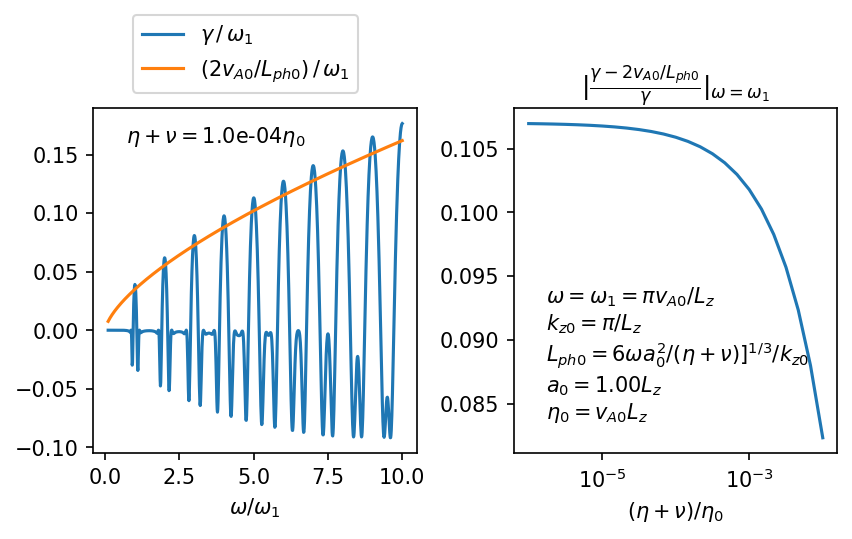
\includegraphics[width=\textwidth,height=0.85\textheight,keepaspectratio]{figures/chapter03/closed_loop_gamma.png}
    \vspace{-30pt}
    \caption{This figure shows plots of the heating rate per unit of wave energy, $\gamma$. The left-hand side shows $\gamma$ as a function of frequency. The blue and orange curves were calculated using Equations \eqref{eq:gamma_exact_closed_loop} and \eqref{eq:gamma_approx_closed_loop} respectively. The right-hand side shows the relative error between these two equations as a function of $(\eta+\nu)$. The code used to make this figure is available on GitHub in the following directory:\newline
    \texttt{$\rightarrow$ Python/Chapter3/closed\_loop\_gamma.py}}
    \label{fig:closed_loop_gamma}
    \vspace{-10pt}
\end{figure}

Our goal now is to verify that Equation \eqref{eq:gamma_approx_closed_loop} provides an approximation for Equation \eqref{eq:gamma_exact_closed_loop} on resonant field lines. Also, we aim to calculate $\gamma$ for the non-resonant field lines. To do this, we take a graphical approach. In Figure \ref{fig:closed_loop_gamma} we present $\gamma$. The blue and orange curves on the left-hand side show $\gamma$ as a function of $\omega$ and were calculated using Equations \eqref{eq:gamma_exact_closed_loop} and \eqref{eq:gamma_approx_closed_loop} respectively. The blue curve shows that $\gamma$ is largest at the resonant frequencies and is significantly smaller away from the resonance and can even be negative. The solution can be negative, and this is because we approximate $\gamma$ here using the Poynting flux instead of the heating rate. Therefore the energy injected into a field line at $z=0$ can be transferred to neighbouring field lines due to diffusion. At first, it may seem surprising that $\gamma$ is so small at non-resonant frequencies because the wave energy, which appears on the denominator of Equation \eqref{eq:gamma_exact_closed_loop}, decreases as the frequency moves away from the resonant frequencies. However, the numerator decreases to a greater degree as the frequency shifts away from the resonant frequencies. Typically, waves need to propagate within the loop for a long time before the length-scales in $x$ become short enough for significant heating to occur. At non-resonant frequencies, waves cannot phase-mix to short enough length-scales before they are eliminated due to destructive interference. Note that the timescale for waves to be eliminated is characterised by the beating time, which we studied in Section \ref{sec:case_where_omega_approx_omega_n}. Comparing the blue and orange curves, we see that Equation \eqref{eq:gamma_approx_closed_loop} provides an approximation for Equation \eqref{eq:gamma_exact_closed_loop} at the resonant frequencies. The right-hand side presents the relative error between the two equations at $\omega=\omega_1$ and as a function of $\eta+\nu$. We see that the relative error remains within about 10\%.

\subsection{Multiple harmonics}
\label{sec:chap_3_closed_loop_multiple_harmonics}

We showed in Section \ref{sec:mhd_waves_power_spectrum} that velocity fluctuations oscillate at a broad range of frequencies. In this section, we aim to calculate the heating rate per unit of wave energy, $\gamma$, for the case where the driver excites a broad range of frequencies. In Section \ref{sec:closed_loop_random_driver}, we showed that the power spectrum in a closed loop with a broadband driver will on average have peaks at the resonant frequencies. \citet{Wright1995} have also observed this. Therefore, for simplicity, our driver will only excite the resonant frequencies.

Let the bottom boundary condition be given by
\begin{equation}
    \label{eq:driver_multiple_harmonics}
    \begin{aligned}
    u(x,0,t) &= f_{driv}(t)\\
    &=f_0 \sum_{n=-N}^N C_n \exp(i\omega_n t),
    \end{aligned}
\end{equation}
where
\begin{gather}
    C_n = \begin{dcases}
    0, & n=0, \\
    \frac{\sqrt{L_z} n^{-\alpha / 2}\exp(i\varphi_n)}{\sqrt{\int_0^{L_z} |A_{\infty,n}|^2 + |B_{\infty,n}|^2 dz}}, & n > 0, \\
   \bar{C}_{|n|}, & n < 0,
    \end{dcases} \\
    A_{\infty,n} = \sum_{k=0}^\infty(-1)^k\exp(-ik_{z,n}z_k)\exp[-(z_k / L_{ph,n})], \\
    B_{\infty,n} = \sum_{k=0}^\infty \exp(-ik_{z,n}z_k)\exp[-(z_k / L_{ph,n})], \\
    \omega_n = n\frac{\pi v_{A0}}{L_z}, \\
    k_{z,n} = \frac{\omega_n}{v_{A0}}, \\
    L_{ph,n} = \qty[\frac{6\omega_n a^2}{\eta+\nu}]^{1/3}\frac{1}{k_{z,n}}.
\end{gather}
Note that $\alpha$ controls the slope of the power spectrum, $\varphi_n\in\mathds{R}$ gives an arbitrary phase, $\bar{C}_{|n|}$ denotes the complex conjugate and ensures the driver is real and $N$ controls the number of harmonics which are excited. From Equations \eqref{eq:chap_3_closed_loop_phase_mix_soln_u} and \eqref{eq:chap_3_closed_loop_phase_mix_soln_b} we know that the steady-state solutions are given by
\begin{gather}
    u(x,z,t) = f_0\sum_{n=-N}^NA_{\infty,n}C_n\exp(i\omega_n t), \\
    b(x,z,t) = -B_0\frac{f_0}{v_A}\sum_{n=-N}^NB_{\infty,n}C_n\exp(i\omega_n t).
\end{gather}

By Parsvel's theorem, the time-averaged energy is given by
\begin{equation}
    \begin{aligned}
    \langle e_\infty \rangle &=\frac{1}{P}\int_0^{P}\frac{\rho |u|^2}{4} + \frac{|b|^2}{4\mu}dt
\\&=\frac{B_0^2f_0^2}{4\mu v_A^2}\sum_{n=-N}^N |A_{\infty,n} C_n|^2 + |B_{\infty,n} C_n|^2,
    \end{aligned}
\end{equation}
where
\begin{equation}
    P = \frac{2L_z}{v_{A0}}.
\end{equation}
Therefore, the energy of the whole loop, $\langle E_\infty \rangle$, is given by
\begin{equation}
    \begin{aligned}
    \langle E_\infty \rangle &= \frac{B_0^2f_0^2}{4\mu v_A^2}\sum_{n=-N}^N|C_n|^2\int_0^{L_z}|A_{\infty,n}|^2+|B_{\infty,n}|^2 dz \\
    &= \frac{B_0^2f_0^2}{2\mu v_A^2}L_z\sum_{n=1}^Nn^{-\alpha}.
    \end{aligned}
\end{equation}
The above equations shows that our driver, Equation \eqref{eq:driver_multiple_harmonics}, ensures that the energy of the loop has a power spectrum with slope $\omega_n^{-\alpha}$.

Using Parseval's theorem, the average Poynting flux is given by
\begin{equation}
    \begin{aligned}
    \langle S_z \rangle &= \frac{B_0^2f_0^2}{2\mu v_A}\sum_{n=-N}^N|C_n|^2\Re(A_{\infty,n}\bar{B}_{\infty,n}) \\
    &= \frac{B_0^2f_0^2}{\mu v_A}L_z\sum_{n=1}^Nn^{-\alpha}\frac{\Re(A_{\infty,n}\bar{B}_{\infty,n})}{\int_0^{L_z}|A_{\infty,n}|^2+|B_{\infty,n}|^2dz}.
    \end{aligned}
\end{equation}
Therefore, the heating rate per unit of wave energy, $\gamma$, is given by
\begin{equation}
    \label{eq:gamma_multiple_harmonics_exact}
    \begin{aligned}
    \gamma &= \frac{\langle S_z\rangle|_{z=0}}{\langle E_{\infty} \rangle} \\
    &=\frac{\sum_{n=1}^Nn^{-\alpha}\gamma_n}{\sum_{n=1}^Nn^{-\alpha}},
    \end{aligned}
\end{equation}
where
\begin{equation}
    \gamma_n = 2v_A\frac{\Re(A_{\infty,n}\bar{B}_{\infty,n})|_{z=0}}{\int_0^{L_z}|A_{\infty,n}|^2+|B_{\infty,n}|^2dz}.
\end{equation}
Hence, $\gamma$ takes the form of a weighted average of the set $\{\gamma_n\}$ with weights $n^{-\alpha}$.

Our goal now is to approximate Equation \eqref{eq:gamma_multiple_harmonics_exact} in a more convenient form. We approximate $\gamma_n$ by using Equation \eqref{eq:gamma_approx_closed_loop} to give
\begin{equation}
    \begin{aligned}
    \gamma_n &\approx \omega_n\qty[\frac{4(\eta+\nu)}{3\omega_na^2}]^{1/3} \\
    &= \omega_1\qty[\frac{4(\eta+\nu)}{3\omega_1a^2}]^{1/3}n^{2/3}.
    \end{aligned}
\end{equation}
Hence, Equation \eqref{eq:gamma_multiple_harmonics_exact} can be approximated as
\begin{equation}
    \label{eq:gamma_multiple_harmonics_approx}
    \begin{aligned}
    \gamma &\approx \gamma_1\frac{\sum_{n=1}^Nn^{2/3-\alpha}}{\sum_{n=1}^Nn^{-\alpha}} \\
    &= \gamma_1\frac{H_N^{(\alpha-2/3)}}{H_N^{(\alpha)}},
    \end{aligned}
\end{equation}
where $H_N^{(p)}$ denotes the generalised harmonic number of order $p$ of $n$.
Note that
\begin{equation}
\label{eq:generalised_harmonic_number_approx}
H_N^{(p)}=
    \begin{dcases}
    \ln(N) + \gamma_{EM} + O(1/N), & p=1 \\
    N^{-p}\qty[\frac{N}{1-p}+\frac{1}{2}+O(1/N)] + \zeta(p), & p\ne 1 \\
    \end{dcases}
\end{equation}
where $\zeta(p)$ denotes the Riemann zeta function (see right-side of Figure \ref{fig:multiple_harmonics}) and $\gamma_{EM}$ is the Euler-Mascheroni constant. Hence, 
if $\alpha=0$, then to leading order
\begin{equation}
    \label{eq:gamma_alpha=0}
    \gamma \approx \gamma_1\frac{3N^{2/3}}{5} + O(N^{-1/3}),
\end{equation}
if $\alpha = 1$, then to leading order
\begin{equation}
    \label{eq:gamma_approx_alpha=1}
    \gamma \approx \gamma_1\frac{3N^{2/3}/2+\zeta(1/3) + O(N^{-1/3})}{\ln(N)+\gamma_{EM}+O(1/N)},
\end{equation}
if $\alpha=5/3$, then to leading order
\begin{equation}
    \label{eq:gamma_alpha=5/3}
    \gamma \approx \gamma_1\frac{\ln(N) + \gamma_{EM} + O(1/N)}{\zeta(5/3)+O(N^{-2/3})}.
\end{equation}

Our goal now is to check that $\gamma$, given by Equation \eqref{eq:gamma_multiple_harmonics_exact}, can be approximated with Equation \eqref{eq:gamma_multiple_harmonics_approx} with $H_N^{(p)}$ approximated by Equation \eqref{eq:generalised_harmonic_number_approx}. We test this using a graphical approach. On the left-side of Figure \ref{fig:multiple_harmonics} we plot the heating rate per unit of wave energy, $\gamma$, as a function of the number of excited harmonics, $N$, for different power spectra slopes, $\alpha$. The exact solution (solid line) was calculated using Equation \eqref{eq:gamma_multiple_harmonics_approx}. The approximate solution (`+' symbols), was calculated using \eqref{eq:gamma_multiple_harmonics_exact} with with $H_N^{(p)}$ approximated by Equation \eqref{eq:generalised_harmonic_number_approx}. Note that to account for the error associated with approximating $\gamma$ with Equation \eqref{eq:gamma_approx_closed_loop} we multiply our approximation by a factor 1.1. This factor comes from the fact that we noted an error of about 10\% in Figure \ref{fig:closed_loop_gamma}.
We plot for the case where $\alpha=0$ (blue), $1$ (orange), and $5/3$ (green), these can be approximated with Equations \eqref{eq:gamma_alpha=0}-\eqref{eq:gamma_alpha=5/3} respectively. The plots suggest that our approximation is indeed accurate for $N\gg1$. Note that if the power spectra are steep, $\alpha=5/3$ say, then $\gamma$ is weakly dependent on the number of harmonics. If the power spectra are flatter, $\alpha=0$, then $\gamma$ is highly dependent on the number of excited harmonics.

\begin{figure}
    \centering
    \vspace{-20pt}
    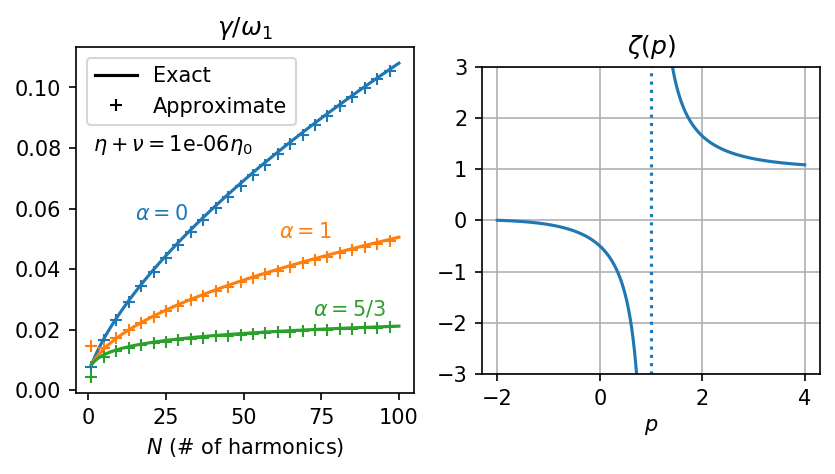
\includegraphics[width=\textwidth,height=0.85\textheight,keepaspectratio]{figures/chapter03/multiple_harmonics.png}
    \vspace{-30pt}
    \caption{This figure shows line plots of the heating rate per unit of wave energy as a function of the number of excited harmonics, $N$, on the left. 
    % The exact solution was calculated using Equation \eqref{eq:gamma_multiple_harmonics_approx}  and the approximate solution was calculated using \eqref{eq:gamma_multiple_harmonics_exact} with with $H_N^{(p)}$ approximated by Equation \eqref{eq:generalised_harmonic_number_approx}. 
    The right-side shows the Riemann zeta function along the real axis where the discontinuity at $p=1$ is denoted with a dotted line. The code used to make this figure is available on GitHub in the following directory:\newline
    \texttt{$\rightarrow$ Python/Chapter3/multiple\_harmonics.py}}
    \vspace{-20pt}
    \label{fig:multiple_harmonics}
\end{figure}

Figure \ref{fig:multiple_harmonics} uses a range of $\alpha$ values including $5/3$ as this is one the values predicted from MHD turbulence theory \citep{Bruno2013}. \citet{Morton2016} provides observations of the power spectra of velocity fluctuations in the quiet sun, the active regions, and the coronal holes (see Figure \ref{fig:power_spectrum_morton}). These latter authors find that the slope varies from $\alpha = 1$ to $\alpha = 1.53$ for higher frequencies, although they are only able to measure up to frequencies of around $10^{-2}\si{.Hz}$. \citet{Podesta2007} measure the power spectra in the solar wind and can measure up to $10^{-1}\si{.Hz}$ and find the slope to be between $\alpha = 1.5$ $\alpha = 5/3$.

\section{Leaky loop}
\label{sec:chap_3_leaky_loop}

In Section \ref{sec:leaky_loop_reflection_coefficent}, we showed that waves can leak out of the corona. In this section, we aim to study phase-mixed Alfv\'en waves in a leaky loop and calculate the effects of leakage on the value of $\gamma$. We use similar boundary conditions to those used in Section \ref{sec:leaky_loop_general_solution}, namely, 
\begin{equation}
    \tag{\ref{eq:bcs_elsasser}}
    \begin{aligned}
    \mathcal{Z}^{-}(x,0,t) &= 2f_{driv}(x,t) - R\mathcal{Z}^+(x,0,t) \\
    \mathcal{Z}^{+}(x,L_z,t) &= -R\mathcal{Z}^-(x,L_z,t),
    \end{aligned}
\end{equation}
where $R$ gives the reflection coefficient, which we approximate in Section \ref{sec:leaky_loop_reflection_coefficent}. These boundary conditions ensure that each time a wave reaches a boundary a fraction $R$ of the wave is reflected and a fraction $1-R$ leaks out of the loop.

Our first goal is to calculate the timescale at which waves decay due to leakage. We will compare this with the resisitive timescale to estimate the parameter space in which leakage plays a significant role in the decay of waves compared with resistive effects. Consider an ideal loop. The time taken for a wave to travel from $z=0$ to $z=L_z$ (and vice versa) is the Alfv\'en travel time, $\tau_A$, given by
\begin{equation}
    \label{eq:chap_3_alfven_travel_time}
    \tau_A = \frac{L_z}{v_A}.
\end{equation}
Therefore each time $\tau_A$ time units have elapsed the wave amplitude decreases by $R$. Thus, the wave amplitude, $u_0$, goes as
\begin{equation}
    \begin{aligned}
    u_0 &\propto R^{\lfloor t / t_{A} \rfloor} \\
    &= \exp\qty(\left\lfloor\frac{t}{t_A}\right\rfloor\ln R) \\
    &\approx \exp\qty(-\frac{|\ln R|}{t_A}t).
    \end{aligned}
\end{equation}
Hence, the leakage timescale, $\tau_{leakage}$, is given by,
\begin{equation}
    \tau_{leakage} = \frac{L_z}{v_A |\ln R|}.
\end{equation}
Each time a wave propagates a distance, $L_{ph}$, the wave decays by a factor $\exp(1)$ due to resistive effects. Therefore, the resistive timescale is given by 
\begin{equation}
\begin{aligned}
    \tau_{resistive} &= \frac{L_{ph}}{v_A} \\
    &= \qty[\frac{6\omega^2a^2}{\eta+\nu}]^{1/3}\frac{1}{\omega}.
\end{aligned}
\end{equation}
If $\tau_{resistive}\ll\tau_{leakage}$ then we expect leakage to play a negligible role and the solution to be well approximated by our calculation in Section \ref{sec:chap_3_closed_loop}. If $\tau_{resistive}\ll\tau_{leakage}$ then we expect resistivity and viscosity to play negligible role in determining the shape of the solution, however, any heating which occurs will still be Ohmic and viscous. To get an idea of the parameter space in which leakage plays an important we plot $\tau_{resistive}$ and $\tau_{leakage}$ on the left-hand side of Figure \ref{fig:chap_3_leaky_loop} as a function of $f$ in $\si{Hz}$. The plot shows that the leakage timescale is smaller than the resistive timescale for this parameter space. We show our choice of parameters in the figure, e.g. we assume a background Alfv\'en speed of $10^6\si{.m.s^{-1}}$, where we chose the parameters to represent typical values in coronal loops.

\begin{figure}
    \vspace{-20pt}
    \centering
    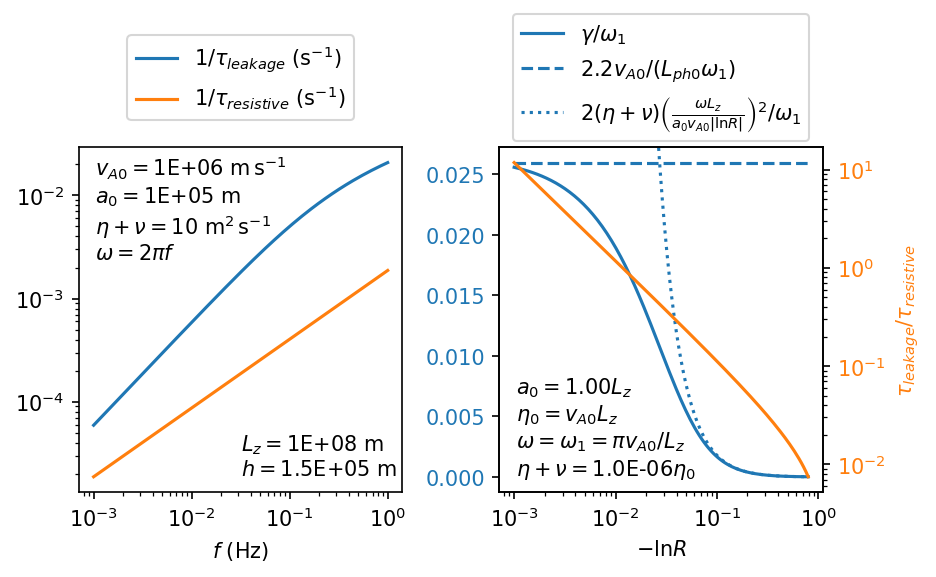
\includegraphics[width=\textwidth,height=0.85\textheight,keepaspectratio]{figures/chapter03/leaky_loop.png}
    \vspace{-35pt}
    \caption{This figure shows plots of the leakage timescale, $\tau_{leakage}$, and resistive timescale, $\tau_{resistive}$ on the left as a function of the wave frequency. The right-side shows $\gamma$ in blue and the ratio, $\tau_{leakage}/\tau_{resistive}$, in orange, as a function of the reflection coefficient, R. The code used to make this figure is available on GitHub in the following directory:\newline
    \texttt{$\rightarrow$ Python/Chapter3/leaky\_loop.py}}
    \label{fig:chap_3_leaky_loop}
    \vspace{-15pt}
\end{figure}

Extending Equations \eqref{eq:chap_3_closed_loop_phase_mix_soln_u} and \eqref{eq:chap_3_closed_loop_phase_mix_soln_b} to include leakage gives
\begin{gather}
\label{eq:chap_3_full_soln_leaky_resistive_u}
\begin{aligned}
    u(x,z) &= f_0\sum_{k=0}^\infty(-1)^kR^k\exp[-ik_z(x)z_k]\exp[-(z_k/L_{ph})^3] \\
    &= f_0A_\infty'(x,z),
\end{aligned}
\\
\begin{aligned}
    b(x,z) &= -B_0\frac{f_0}{v_A}\sum_{k=0}^\infty R^k\exp[-ik_z(x)z_k]\exp[-(z_k/L_{ph})^3] \\
    &= -B_0\frac{f_0}{v_A}B_\infty'(x,z),
\end{aligned}
\end{gather}
where
\begin{gather}
    A_\infty'(x,z) = \sum_{k=0}^\infty(-1)^kR^k\exp[-ik_z(x)z_k]\exp[-(z_k/L_{ph})^3], \\
    B_\infty'(x,z) = \sum_{k=0}^\infty R^k\exp[-ik_z(x)z_k]\exp[-(z_k/L_{ph})^3].
\end{gather}
Introducing leakage means that the Poynting flux at $z=L_z$ is no longer necessarily equal to zero, therefore, the heating rate per unit of wave energy is given by
\begin{equation}
    \label{eq:gamma_exact_leaky_loop}
    \gamma(x) = -2v_A\frac{[\Re(A_\infty'\bar{B}_\infty')]_{z=0}^{z=L_z}}{\int_0^{L_z}|A_\infty'|^2+|B_\infty'|^2dz)}.
\end{equation}

The above equation for $\gamma$ is quite cumbersome because it is difficult to see its dependency on parameters such as $\omega$ or $R$. Our goal now is to calculate an approximate solution for the case where $\tau_{leakage}\ll \tau_{resistive}$. Note that Equation \eqref{eq:gamma_approx_closed_loop} gives an approximate solution for $\tau_{leakage}\gg \tau_{resistive}$. The heating rate per unit of wave energy, $\gamma$, is approximated by
\begin{equation}
    \begin{aligned}
    \gamma &\approx \frac{\frac{1}{2}(\eta+\nu)\int_0^{L_z}\rho (\pdv*{u}{x})^2 + (\pdv*{b}{x})^2/\mu dz}{\frac{1}{2}\int_0^{L_z}\rho u^2 + b^2/\mu dz} \\
    &\approx (\eta+\nu)(k_x^*)^2,
    \end{aligned}
\end{equation}
where $k_x^*$ gives a measure of the wavenumber in the $x$-direction. Substituting $z=v_A t$, we estimate $k_x^*$ in the strong leakage limit as
\begin{equation}
\begin{aligned}
    k_x^* &\approx \frac{\omega}{a}\tau_{leakage} \\
    &=\frac{\omega L_z}{a v_A |\ln R|}.
\end{aligned}
\end{equation}
Therefore,in the strong leakage limit,
\[
    \gamma \propto (\eta + \nu)\qty(\frac{\omega L_z}{a v_A |\ln R|})^2.
\]
Note that the dotted curve in Figure \ref{fig:chap_3_leaky_loop} uses
\begin{equation}
    \label{eq:gamma_approx_leaky_loop}
    \gamma = 2(\eta + \nu)\qty(\frac{\omega L_z}{a v_A |\ln R|})^2.
\end{equation}

We now need to plot $\gamma$, given by Equation \eqref{eq:gamma_exact_leaky_loop}, as a function of $R$, to see how leakage affects $\gamma$ and to check the accuracy of Equation \eqref{eq:gamma_approx_leaky_loop}. The solid blue curve on the right-hand side of Figure \ref{fig:chap_3_leaky_loop} shows $\gamma$ as a function of the reflection coefficient $-\ln R$. The plot shows that increasing the leakage (decreasing $R$) causes $\gamma$ to decrease. This is because the leakage reduces the development of short length-scales as waves leak out of the loop before they can phase-mix to the same length-scales that closed-loop waves can reach. The Figure shows that in the limit $\tau_{leakage} / \tau_{resistive} \ll 1$, then $\gamma$ can be approximated with Equation \eqref{eq:gamma_approx_leaky_loop}, where the ratio $\tau_{leakage} / \tau_{resistive}$, is plotted in orange and the approximation is plotted with a dotted blue line. In the limit $\tau_{leakage} / \tau_{resistive} \gg 1$ then $\gamma$ can be well approximated by assuming the loop is closed.

\section{Coronal heating discussion}
\label{sec:chap_3_coronal_heating}

In Section \ref{sec:chap_3_introduction} we showed that we require $\gamma\approx10^{-1}\si{.s^{-1}}$, see Equation \eqref{eq:required_gamma}, for phase mixing to play an important role in coronal heating. Our goal now is to use results from Sections \ref{sec:chap_3_closed_loop}-\ref{sec:chap_3_leaky_loop} to estimate an upper bound for a typical value of $\gamma$ in the closed corona using phase-mixing theory. We will first present our estimate. After that, we will discuss some of our simplifications and calculate if they increase or decrease our estimate of $\gamma$.

In Section \ref{sec:chap_3_closed_loop_heating_rate} we showed that if a single harmonic is excited, then $\gamma$ can be well approximated with Equation \eqref{eq:gamma_approx_closed_loop}. Velocity fluctuations in the corona typically oscillate at a superposition of multiple frequencies, with a power spectrum approximated by Figure \ref{fig:power_spectrum_morton}. In Section \ref{sec:chap_3_closed_loop_multiple_harmonics}, we showed if multiple harmonics are excited and have a power spectrum proportional to $f^{-\alpha}$, where $f$ denotes the frequency of the waves, then $\gamma$ is approximated with Equation \eqref{eq:gamma_multiple_harmonics_approx}. Substituting for typical values, with $\alpha=1$, $N=100$, Equation \eqref{eq:gamma_approx_alpha=1} gives
\begin{equation}
    \label{eq:upper_bound_for_gammma}
    \gamma \approx 1.43\times10^{-4} \qty(\frac{\omega_1}{\pi\times10^{-2}\si{.Hz}})^{1/3}\qty(\frac{\eta+\nu}{10\si{.m^2.s^{-1}}})^{1/3}\qty(\frac{1\si{.Mm}}{a})^{2/3}\si{.s^{-1}}.
\end{equation}
Therefore, our upper bound for $\gamma$ is significantly less than the required value of $\gamma$, by approximately three orders of magnitude. This implies that the $\vec{W}^{(1)}$ component of the viscosity tensor, $\vec{\sigma}_{Brag}$, plays a negligible role in coronal heating. This suggests that the direct dissipation of waves due to the steep gradients generated by phase-mixing play an insignificant role in coronal heating. However, phase mixing could still play an important but less direct role in coronal heating. For example, phase mixed Alfv\'en waves are susceptible to the Kelvin-Helmholtz and tearing mode instabilities, leading to a turbulent cascade to smaller scales. This would mean that the dissipation occurs primarily due to gradients parallel to the field or the velocity which are dissipated via the $\vec{W}^{(0)}$ component of the viscosity tensor. Note that $\vec{W}^{(0)}$ is not dependent on the gradients generated through phase-mixing since the $x$-direction is neither parallel to the field or the velocity. In \citet{Hillier2019} they show that the Kelvin-Helmholtz instability can lead to coronal cooling as a result of the fluid mixing together which causes the temperate to become more uniform resulting in the total amount of radiation increases. To derive the above equations, we had to make several simplifications. The rest of this section justifies these simplifications and explains why we chose the values for the above parameters.

Increasing $\alpha$ acts to reduce $\gamma$. For our calculation we took $\alpha=1$, which underestimates the single power-law fit to Figure \ref{fig:power_spectrum_morton}. This helps ensure that our calculation for $\gamma$ is an upper bound. We chose $N=100$ because $100\omega = \pi\si{.Hz}$ which is a higher than the maximum observed wave frequencies. We will also show later, in Equation \eqref{eq:w01}, for high frequencies, phase mixing plays a negligible role in the dissipation of waves compared with the dissipation due to gradients parallel to the background field. The characteristic length of a coronal loop is about $100\si{.Mm}$ \citep{O'Neill2005} with an average Alfv\'en speed of about $1\si{.Mm.s^{-1}}$ \citep{McIntosh2011}. This gives a fundamental angular frequency of $\omega_1=\pi\times10^{-2}\si{.Hz}$. Combining Equations \eqref{eq:braginskii_eta_1} and \eqref{eq:proton_gyrofrequency_times_collision_time} gives
\begin{equation}
    \label{eq:nu_typical_values}
    \nu=\frac{\eta_1}{\rho} = 1.38\,\qty(\frac{10^{-3}\si{.Tesla}}{B_0})^2\qty(\frac{10^6\si{.K}}{T})^{1/2}\qty(\frac{\rho}{10^{-12}\si{.kg.m^{-3}}})\si{.m^2.s^{-1}},
\end{equation}
where the Coulomb logarithm, $\log\Lambda$, has been set equal to $20$. Therefore, Equations \eqref{eq:eta_typical_values} and \eqref{eq:nu_typical_values} show that $\eta+\nu<10\si{.m^2.s^{-1}}$ for the given set of parameters. The parameter with the greatest level of uncertainty associated with it is the length-scale of the Alfv\'en travel times, $a$, given by Equation \eqref{eq:length_scale_alfven_travel_time}. We discuss a suitable value for $a$ in the next paragraph. 

Three factors determine the Alfv\'en travel time of a loop, the length of the loop, the plasma density, and the magnetic field strength. In \citet{Oliver1993}, they calculate the Alfv\'en travel time in a potential coronal arcade with a uniform density profile. The flux function, $A$, is given by
\begin{equation}
    \label{eq:potential_aracde_flux_function}
    A(x,z) = B_0\Lambda_B\cos(\frac{x}{\Lambda_B})\exp(-\frac{z}{\Lambda_B}),
\end{equation}
where $B_0$ gives the field strength at $z=0$, $\Lambda_B$ gives the scale height of the field strength and is also related to the arcade's lateral extent. Note that lines of constant $A$ provide the field lines and the associated magnetic field is given by $\vec{B}=\grad{A}\cross\vec{\hat{y}}$. We plot the field on the left side of Figure \ref{fig:potential_arcade}. In \citet{Oliver1993} they show that the fundamental frequency of this arcade is given by
\begin{equation}
    \omega_1 = \pi\frac{v_{A0}}{2x_0}\cos(\frac{x_0}{\Lambda_B}),
\end{equation}
where $v_{A0}$ gives the Alfv\'en speed at $z=0$ and $x_0$ gives the $x$-coordinate of the field line at $z=0$. Therefore, the length-scale of Alfv\'en travel time variations across the field lines can be approximated with
\begin{equation}
    \begin{aligned}
    a(x_0) &= \abs{\frac{\omega_1}{\dv*{\omega_1}{x_0}}} \\
    &= \frac{x_0\Lambda_B\cos(x_0/\Lambda_B)}{\Lambda_B\cos(x_0/\Lambda_B)+x_0\sin(x_0/\Lambda_B)}.
    \end{aligned}
\end{equation}
Note that $a(x_0)$ is plotted on the right-side of Figure \ref{fig:potential_arcade}. The plot shows that $a = 0$ for $x_0=0$ and $x_0=\pi\Lambda_B/2$.  The magnetic field lines are highly divergent near $x_0=\pi\Lambda_B/2$. It has been shown in for example \citet{Smith2007} that a diverging field can enhance the phase mixing. However, we are interested in an average value for $a$. The average value, $\langle a \rangle$ is given by
\begin{equation}
\begin{aligned}
    \langle a(x_0) \rangle &= \frac{2}{\pi\Lambda_B}\int_0^{\pi\Lambda_B/2}a(x_0)dx_0 \\
    &= \frac{2}{\pi}\ln(\frac{\pi}{2})\Lambda_B \\
    &\approx 2.87\qty(\frac{\Lambda_B}{10\si{.Mm}}) \si{.Mm}.
\end{aligned}
\end{equation}
For $x_0\rightarrow0$, $\omega_1\rightarrow\infty$. Therefore, a resonance near $x_0=0$ must have a very high frequency. Figure \ref{fig:reflection_coefficent} showed that very high frequencies can leak into the chromosphere more easily. This suggests imposing solid boundary conditions may not be appropriate here.
The Alfv\'en travel time is also affected by the density of the plasma. \citet{Klimchuk2015} shows that coronal loops have a characteristic diameter of approximately $1.5\si{.Mm}$. If we assume a density contrast, $\rho_i/\rho_o=2$, \citep{Hood2013,Pascoe2013} where $\rho_i$ gives the density inside a loop and $\rho_o$ gives the density outside a loop then this gives a length-scale $a\approx750\si{.km}$.

\begin{figure}
    \centering
    \vspace{-20pt}
    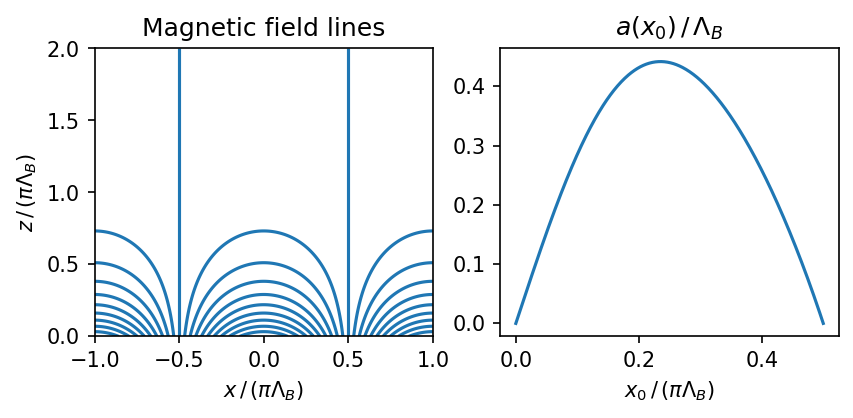
\includegraphics[width=\textwidth,height=0.8\textheight,keepaspectratio]{figures/chapter03/potential_arcade.png}
    \vspace{-30pt}
    \caption{This figure's left side shows a plot of the magnetic field lines where the flux function is given by Equation \eqref{eq:potential_aracde_flux_function}. The right side shows plots of $a$ for the field lines as a function of the footpoint coordinate, $x_0$. The code used to make this figure is available on GitHub in the following directory:\newline
    \texttt{$\rightarrow$ Python/Chapter3/potential\_arcade.py}}
    \vspace{-10pt}
    \label{fig:potential_arcade}
\end{figure}

We modelled the system as linear. This meant the $\vec{W}^{(0)}$ component of the viscosity was neglected. If we assume $\vec{u}=u(x,z,t)\vec{\hat{y}}$ and $\vec{B}=B_0\vec{\hat{z}} + b(x,z,t)\vec{\hat{y}}$ and don't linearise, then
\begin{equation}
    \eta_0\vec{W}^{(0)}:\grad{\vec{u}} = 3\eta_0\epsilon^2\qty(\pdv{u}{z})^2 + O(\epsilon^3),
\end{equation}
where $\epsilon=u/v_A$.
Therefore, the ratio, $w_{0,1}$, between the heating generated by $\vec{W}^{(0)}$ and $\vec{W}^{(1)}$ can be estimated. For simplicity we choose $\eta=0$, hence,
\begin{equation}
\label{eq:w01}
\begin{aligned}
    w_{0,1} &= \frac{\eta_0\vec{W}^{(0)}:\grad{\vec{u}}}{\eta_1\vec{W}^{(1)}:\grad{\vec{u}}} \\
    &\approx 3\epsilon^2\frac{\eta_0}{\eta_1}\qty(\frac{k_z}{k_x^*})^2 \\
    &\approx 4.0471\times10^{-6}\frac{e^{2/3}\mu}{(\ln\Lambda)^{4/3}}\epsilon^2\frac{T^{8/9}\omega^{4/3}}{\rho^{1/3}B_0^{4/3}}a^{2/3} \\
    &\approx 0.59\times10^{-2}\qty(\frac{\epsilon}{10^{-1}})^2\qty(\frac{T}{10^{6}\si{.K}})^{8/9}\qty(\frac{\omega}{\pi\times10^{-2}\si{.Hz}})^{4/3}\\
    &\times\qty(\frac{10^{-12}\si{.kg.m^{-3}}}{\rho})^{1/3}\qty(\frac{10^{-3}\si{.T}}{B_0})^{4/3}\qty(\frac{a}{10^5\si{.m}})^{2/3},
\end{aligned}
\end{equation}
where $k_x^*$ is given by Equation \eqref{eq:phase_mixed_x_length_scale}.

Another consequence of linearising the system is that it causes the Alfv\'en waves to become decoupled from the fast and slow waves. To see this, consider the $y$-component of the ideal momentum equation, Equation \eqref{eq:momentum}, with gravity neglected, $\pdv*{}{y}=0$ and multiplied by $v_y=u$,
\begin{equation}
    \rho\pdv{}{t}\qty(\frac{1}{2}v_y^2)+\rho\vec{v}\vdot\grad\qty(\frac{1}{2}v_y^2)=(\vec{B}\vdot\grad)B_y,
\end{equation}
where $B_y=b$.
Consider the the mass continuity equation, Equation \eqref{eq:mass_continuity}, multiplied by $v_y^2/2$ to give 
\begin{equation}
    \frac{1}{2}v_y^2\pdv{\rho}{t}+\frac{1}{2}v_y^2\div(\rho\vec{v})=0.
\end{equation}
Combining the above equations gives the equation for the evolution of the Alfv\'en wave kinetic energy,
\begin{equation}
    \label{eq:nonlinear_alfven_wave_kinetic_energy}
    \pdv{}{t}\qty(\frac{1}{2}\rho v_y^2) + \div(\frac{1}{2}\rho v_y^2\vec{v})=\frac{1}{\mu}v_y(\vec{B}\vdot\grad)B_y.
\end{equation}
Taking the dot product of Faraday's Law, Equation \eqref{eq:faradays_law}, with $\vec{B}_y/\mu=B_y/\mu\vec{\hat{y}}$, gives
\begin{equation}
    \begin{aligned}
    \pdv{}{t}\qty(\frac{B_y^2}{2\mu})&=-\frac{\vec{B}_y}{\mu}\vdot\curl{\vec{E}} \\
    &=-\div(\frac{\vec{E}\cross\vec{B}_y}{\mu})-\vec{E}\vdot\qty(\frac{\curl{\vec{B}_y}}{\mu}).
    \end{aligned}
\end{equation}
Substituting the ideal Ohms law, Equation \eqref{eq:ohms_law}, gives the equation for the evolution of the Alfv\'en wave magnetic energy
\begin{equation}
    \label{eq:nonlinear_alfven_wave_magnetic_energy}
    \begin{aligned}
     \pdv{}{t}\qty(\frac{B_y^2}{2\mu}) + \div(\frac{\vec{E}\cross\vec{B}_y}{\mu}) &= -\frac{1}{\mu}\vec{v}\vdot[(\curl{\vec{B}_y})\cross\vec{B}] \\
     &=-\frac{1}{\mu}v_y(\vec{B}\vdot\grad)B_y + \vec{v}\vdot\grad\qty(\frac{B_y^2}{2\mu}) \\
    \end{aligned}
\end{equation}
Superimposing Equations \eqref{eq:nonlinear_alfven_wave_kinetic_energy} and \eqref{eq:nonlinear_alfven_wave_magnetic_energy} gives the equation for the energy evolution of the Alfv\'en waves
\begin{equation}
    \pdv{}{t}\qty(\frac{1}{2}\rho v_y^2 + \frac{B_y^2}{2\mu}) + \div(\frac{1}{2}\rho v_y^2 \vec{v} + \frac{\vec{E}\cross\vec{B}_y}{\mu})=\vec{v}\vdot\grad(\frac{B_y^2}{2\mu}).
\end{equation}
The above equation shows that the energy associated with perturbations in the $y$-direction (the Alfv\'en wave) is coupled to the perturbations in the $x$ and $z$ direction through the ponderomotive force, $-\grad[B_y^2/(2\mu)]$. The ponderomotive force is defined as the magnetic pressure force associated with the Alfv\'en wave \citep{Verwichte1999}. In \citet{Verwichte1999} they show that each time nonlinear Alfv\'en pulses pass through each other, they generate a slow magnetoacoustic wave (in $\beta\ll1$ plasma). They also show that for nonlinear Alfv\'en pulses, the Alfv\'en speed is dependent on the wave amplitude. They show that the evolution of an Alfv\'en pulse is described by the Cohen-Kulsrud equation \citep{Cohen1974}, which is similar to Burger's equation. They show that shocks form and calculate the time at which the gradient of the solution becomes singular. \citet{Thurgood2013a,Thurgood2013b} shows that if there are gradients perpendicular to the field and the invariant direction then fast waves are produced by the ponderomotive force. \citet{Terradas2006} show that for a line-tied standing Alfv\'en wave, the ponderomotive force pushes plasma towards the antinodes and away from the nodes. They show that in a $\beta=0$, isothermal, plasma, the amplitude of the density structures grows quadratically with time and this growth is limited by the pressure force if $\beta\ne0$. In \citet{Prokopyszyn2019a}, we investigated standing nonlinear Alfv\'en waves in an x-type null point. We found that introducing nonlinearities had a relatively small effect ($<$10\%) effect on $\gamma$. However, we used an unphysically large value for the diffusion constants to keep the system well resolved numerically.

Modelling the plasma as linear and modelling $\pdv*{}{y}=0$ prevents the development of turbulence through the Kelvin-Helmholtz instability, tearing mode instability and by the nonlinear interaction of counter-propagating Alfv\'en waves \citep{Hollweg1986a,vanBallegooijen2011,Shoda2019}. Turbulence leads to the transfer of energy into higher wavenumbers/frequencies, which causes $\gamma$ to increase. However, we showed in Equation \eqref{eq:w01} that for frequencies greater than about $\omega=\pi\si{.Hz}$ the $\vec{W}^{(0)}$ component of the viscosity tensor starts to dominate. Therefore, our claim that the $\vec{W}^{(1)}$ component plays a negligible role in coronal heating, in general, holds for a turbulent plasma.

Finally, we modelled the plasma as isothermal, and we discuss this in Section \ref{sec:internal_energy_equation}. In \citet{Cargill2016}, they investigate the plasma's thermodynamic response to the heating generated by phase-mixing. They find that the thermodynamics act to reduce the gradient in Alfv\'en speed which reduces $\gamma$. Also, including the thermodynamics will cause the natural frequencies of the system to change with time. \citet{Arregui2015} argues that resonances could not last long enough for substantial heating from phase-mixing to occur. This suggests that including the thermodynamics in the model acts to reduce $\gamma$, which helps ensure Equation \eqref{eq:upper_bound_for_gammma} is an upper bound for $\gamma$.

\section{Conclusions}

The results and discussions in this chapter suggest that the dissipation of the gradients produced by phase mixing plays a negligible role in coronal heating. However, it is possible that phase mixing could trigger the Kelvin-Helmholtz and tearing mode instabilities which cause a turbulent cascade. Then dissipation can occur primarily due to the $\vec{W}^{(0)}$ component of the viscosity tensor which dissipates gradients parallel to the magnetic and velocity fields. In Section \ref{sec:chap_3_introduction} we showed that we require $\gamma\approx10^{-1}\si{.s^{-1}}$ and Equation \eqref{eq:upper_bound_for_gammma} shows that our upper bound for $\gamma$ is too small by approximately 3 orders of magnitude. This upper bound was modelled to be an average upper bound across the whole corona. Phase mixing models can give a larger value of $\gamma$ near, for example, null points or at highly divergent magnetic fields due to the greater presence of viscosity and the Alfv\'en speed-length scale, $a$, being larger.

In Section \ref{sec:chap_3_open_loop} we calculated the solution for a phase-mixed resistive Alfv\'en wave in an open-loop using the method of multiple scales. We then verified this numerically via a graphical approach, see Figure \ref{fig:phase_mxing_open_loop}. We showed that the wave decays with a cubic Gaussian, $\exp[-(z/L_{ph})^3]$, in $z$ with a length scale $L_{ph}$ given by Equation \eqref{eq:phase_mixed_z_length_scale}. This shows that as the wave propagates a larger fraction of the wave decays faster due to the wave phase mixing and the length-scales across the field getting shorter. We estimate at $z=L_{ph}$ the length scales in $x$ are given by Equation \eqref{eq:phase_mixed_x_length_scale}, and we find this is still sufficiently long for collisional transport theory to be valid in the corona. \citet{Heyvaerts1983} shows that propagating Alfv\'en are stable to the Kelvin-Helmholtz instability because the magnetic field and velocity perturbations are in phase with each other. For standing Alfv\'en waves, the velocity and magnetic field perturbations are out of phase with each other in space and time. So the magnetic field cannot stabilise the velocity shear from the Kelvin-Helmholtz instability.

In Section \ref{sec:chap_3_closed_loop} we extended our analytic solution from Section \ref{sec:chap_3_open_loop} to calculate an analytic solution for a closed-loop using a method of images approach. We then verified this numerically and plotted the results in Figure \ref{fig:phase_mixing_closed_loop}. After that, we calculated the solution for the case where multiple harmonics are excited. We showed that an upper bound for the heating rate per unit of wave energy, $\gamma$, can be well approximated with Equation \eqref{eq:gamma_approx_alpha=1} where this assumes a power spectrum with slope $\alpha=1$. We use this formula in Section \ref{sec:chap_3_coronal_heating} to conclude that dissipation of the gradients produced by phase mixing plays a negligible role in coronal heating.

In Section \ref{sec:chap_3_leaky_loop}, we calculate the solution for the case where waves can leak out of the corona. We find that this acts to reduce $\gamma$, and this is because waves leak out of the corona before they can phase-mix to short length scales where significant heating happens. This means that our upper bound for $\gamma$ can ignore the effects of leakage.

Finally, in Section \ref{sec:chap_3_coronal_heating} we brought results from the previous sections to conclude that the dissipation of the gradients produced by phase mixed Alfv\'en plays a negligible role in coronal heating. We then discussed the validity of this conclusion and whether we have missed any essential physics in our model, which might change our judgment. This included: whether our value for the characteristic Alfv\'en speed length-scale, $a$, was valid. Whether unobserved high-frequency waves could be significant. The importance of nonlinearities. The implications of assuming $\pdv*{}{y}=0$. 
Finally, how including the thermodynamic response of the system may affect the results.

% We showed that there is a high level of uncertainty with regards to choosing a characteristic value for the Alfv\'en speed length scale of $a$. By considering an arcade field and observations of the transverse density profile in coronal loops we argued that the value of $a$ we used in Equation \eqref{eq:upper_bound_for_gammma} to be approximately characteristic for the corona to within an order of magnitude. Unobserved very high-frequency waves could play an important role in coronal heating, however, we show that for high-frequency waves the viscous heating due to gradients parallel to the magnetic field and velocity starts to dominate over the heating due to the gradients formed by phase mixing. We neglected nonlinear effects and argued that including nonlinear effects will most likely diminish the importance of phase mixing as the parallel viscosity tensor, $\vec{W}^{0}$, will become more important. We considered the possibility of turbul